\documentclass[border=5pt]{standalone}
\usepackage[utf8]{inputenc}
\usepackage[T1]{fontenc}
\usepackage{tikz}
\usetikzlibrary{arrows.meta, positioning}
\begin{document}
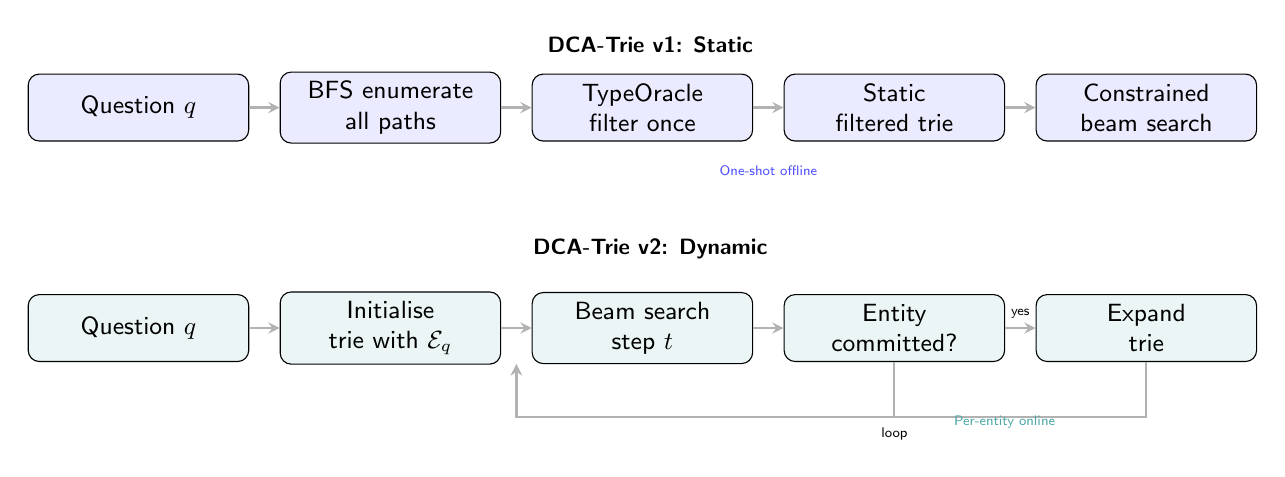
\begin{tikzpicture}[
  >=stealth, font=\sffamily,
  box/.style={draw, rounded corners, minimum width=2.8cm, minimum height=0.85cm,
    align=center, font=\sffamily\small},
  v1box/.style={box, fill=blue!8},
  v2box/.style={box, fill=teal!8},
  arr/.style={->, thick, draw=gray!60},
]

  % v1 pipeline
  \node[font=\sffamily\footnotesize\bfseries] at (6.5, 1.8) {DCA-Trie v1: Static};
  \node[v1box] (q1) at (0, 1) {Question $q$};
  \node[v1box] (bfs) at (3.2, 1) {BFS enumerate\\all paths};
  \node[v1box] (oracle1) at (6.4, 1) {TypeOracle\\filter once};
  \node[v1box] (trie1) at (9.6, 1) {Static\\filtered trie};
  \node[v1box] (decode1) at (12.8, 1) {Constrained\\beam search};

  \draw[arr] (q1) -- (bfs);
  \draw[arr] (bfs) -- (oracle1);
  \draw[arr] (oracle1) -- (trie1);
  \draw[arr] (trie1) -- (decode1);

  % v2 pipeline
  \node[font=\sffamily\footnotesize\bfseries] at (6.5, -0.8) {DCA-Trie v2: Dynamic};
  \node[v2box] (q2) at (0, -1.8) {Question $q$};
  \node[v2box] (init) at (3.2, -1.8) {Initialise\\trie with $\mathcal{E}_q$};
  \node[v2box] (decode2) at (6.4, -1.8) {Beam search\\step $t$};
  \node[v2box] (entity) at (9.6, -1.8) {Entity\\committed?};
  \node[v2box] (expand) at (12.8, -1.8) {Expand\\trie};

  \draw[arr] (q2) -- (init);
  \draw[arr] (init) -- (decode2);
  \draw[arr] (decode2) -- (entity);
  \draw[arr] (entity) -- node[above, font=\sffamily\tiny] {yes} (expand);
  % Loop: expand -> back to decode2
  \draw[arr] (expand.south) -- ++(0,-0.7) -| node[pos=0.2, below, font=\sffamily\tiny] {loop} ([xshift=-1.6cm]decode2.south);
  % No branch
  \draw[arr] (entity.south) -- ++(0,-0.7) -| ([xshift=-1.6cm]decode2.south);

  % Labels
  \node[font=\sffamily\tiny, text=blue!70, align=center] at (8, 0.2) {One-shot offline};
  \node[font=\sffamily\tiny, text=teal!70, align=center] at (11, -3) {Per-entity online};

\end{tikzpicture}
\end{document}
